\chapter{AllDiff-LS的基础组件和算法框架}\label{chap:method}
本章首先对本文的研究问题进行详细介绍,即如何设计一个高效的求解算法来求解一个包含AllDifferent约束的约束满足问题。
基于以上研究问题,本章介绍了本文提出的适用于AllDifferent约束求解的局部搜索算法。
首先,本章节讨论了使用什么数据结构对约束进行表示,以及如何对约束进行建模。
具体地,算法采用了一个包含两种类型的顶点和边的异构图来表示AllDifferent约束,不是单独处理每个allDifferent约束,而是将它们视为一个整体。
其次,算法采用两个低复杂度的顶点简化规则对图进行化简,以减少不必要的搜索空间。
接下来,算法针对构造的图设计求解算法,提出了分两步选择操作的方法,以及相应的打破平局和禁忌策略。
最后,本文给出算法的整体流程图,并展示了包含AllDifferent约束的CSP是如何被求解的。

\section{问题介绍和求解思路}

% 介绍以AllDifferent约束为主的CSP
本文主要研究以AllDifferent约束为主的CSP问题,这是一类特殊的CSP,其中所有的全局约束由AllDifferent约束组成,但允许出现其他类型的二元约束,使得CSP约束的全部或大部由AllDifferent约束组成。在这类问题中,一个变量或包含它的变量表达式将受到多个AllDifferent约束的共同限制,问题的目标是寻找使得所有约束满足的变量赋值。这类问题的一个主要特点是,由于AllDifferent约束的全局性,解空间的大小会随着问题规模的增大而指数级增长。因此,寻找有效的求解策略和算法以提高求解效率,是研究这类问题的一个重要方向。

使用AllDifferent约束可以编码很多经典的CSP,例如数独、n皇后、All-Interval和各类拉丁方问题。以数独问题为例,问题中每一行、每一列以及每一个宫(3x3的小格子)的数字都需要满足AllDifferent约束,即这些位置上的数字都需要是1到9且互不相同。而除此之外,数独问题没有其他的约束条件。

% 介绍此类CSP的形式化定义
设$\mathcal{P} = (X, D, C)$是一个约束满足问题,其中$C$是约束集。定义$AD(c)$成立,当且仅当$c$是一个AllDifferent约束。取$C_A = \{c |c \in C, AD(c)\}$为问题中所有AllDifferent约束组成的集合,本章节后续部分将主要研究如何获得在该约束集上的可满足赋值。
不失一般性的,在本章节的最后会介绍如何将其他二元约束整合到求解的框架中,从而得到整个CSP的可满足赋值。

% 介绍当前存在的问题
考虑到AllDifferent约束强大的约束力,现有的求解器在解决约束数量和长度不断增加的各种CSP问题时,表现出了性能下降的趋势。
本文注意到在AllDifferent约束中,出现的大部分变量都是用来表示变量表达式的,同一个变量不可避免地会出现在多个约束中,这导致约束之间存在强烈的关联性。
此前,关于AllDifferent约束求解的算法分为两类,一类是借助过滤算法对约束化简后再对问题进行回溯求解,第二类则是通过提前满足AllDifferent约束的方式将约束作为隐含约束处理。
这两种策略都是将问题中的AllDifferent约束分别进行处理,而没有考虑约束之间也存在约束关系。此外,随着约束数量的增多,第二类策略无法处理绝大多数AllDifferent约束,使得策略的有效性会大的折扣。

% 介绍拟采用的求解思路
基于以上观察,本文并没有单独对待每一个AllDifferent约束,而是将它们作为一个整体来处理。本文采用了包含两种类型顶点和边的异构图来表示AllDifferent约束,称为AllDifferent约束图(ACG)。构造这个图的动机来源于针对AllDifferent约束的二元分解,本文在此基础上将变量和变量表达式的概念进行了区分,从而使得此框架可以应用于更为广泛的弧一致性算法。


\section{AllDifferent约束转化为图及其优化}
设$\mathcal{P} = (X, D, C)$是一个约束满足问题,$C_A$是其AllDifferent约束组成的集合。约为了表示该问题,本文引入一个异构图$\mathcal{G}$,称之为\textit{AllDifferent约束图}(AllDifferent Constraint Graph,ACG)。为了方便后续描述,约束中涉及的基本单位是\textit{变量表达式},其中,变量表达式可以是包含加减乘除等操作的复杂表达式,也可以是单位表达式。例如,在约束条件 {\it AllDifferent}$(x_1, x_2+x_3)$ 中,$x_1$ 和 $x_2+x_3$ 都是表达式。异构图的形式化表示如下。

\begin{definition}[\textbf{AllDifferent约束图}]
    异构图被定义为$\mathcal{G} = (V, E)$,其中$V = X\cup NV$,表示顶点集合,其中$NV$指出现在AllDifferent约束中的变量表达式集合。
    $E = E_p \cup E_x$表示边集合,它由两种类型的边表示。
    具体来说,一种类型是变量表达式之间的边,称为\textit{表达边},用$E_p$表示,如果两个变量表达式$p$和$q$出现在同一个AllDifferent约束中,它表示为$(p, q) \in E_p$。
    另一种类型是变量和变量表达式之间的边,用$E_x$表示,如果一个变量表达式$p$包含一个变量$x$,则有$(p, x) \in E_x$。
\end{definition}

AllDifferent约束图的思想是,将全局约束用二元分解分解为多组二元约束的并集,再针对二元约束构成的二元关系以及变量表达式和变量之间的二元关系,构造图结构。
和使用残差图对AllDifferent约束进行表示不同,本文没有引入变量-值这一关系。
通过隐去值域这一信息,ACG得以表示多组AllDifferent约束,从而将所有约束使用一张图进行表示,以施展更强的弧一致性算法。
下面,本文通过一个简单的例子来介绍ACG。

\begin{example}\label{exp:acg}
    给定四个变量$x_1$,$x_2$,$x_3$,$x_4$,其有限值域分别为$\{1, 2, 3\}$,$\{1, 2\}$,$\{2, 3\}$和$\{1, 2, 3\}$。
    如果要求$x_1, x_2$和$x_3-1$的赋值不能相同,并且要求$x_1+x_2$和$x_3+x_4$的赋值不能相同,那么可以如下建模此问题:
        \begin{align}
            &\texttt {AllDifferent} (x_1, x_2, x_3-1), & \\
            &\texttt {AllDifferent} (x_1+x_2, x_3+x_4), &
        \end{align}%
    容易看出,该问题的一个解是$\mathcal{A}=(3, 1, 3, 2)$。它的ACG如图\ref{fig:acg}所示。
\end{example}

\begin{figure*}[]
    \centering
    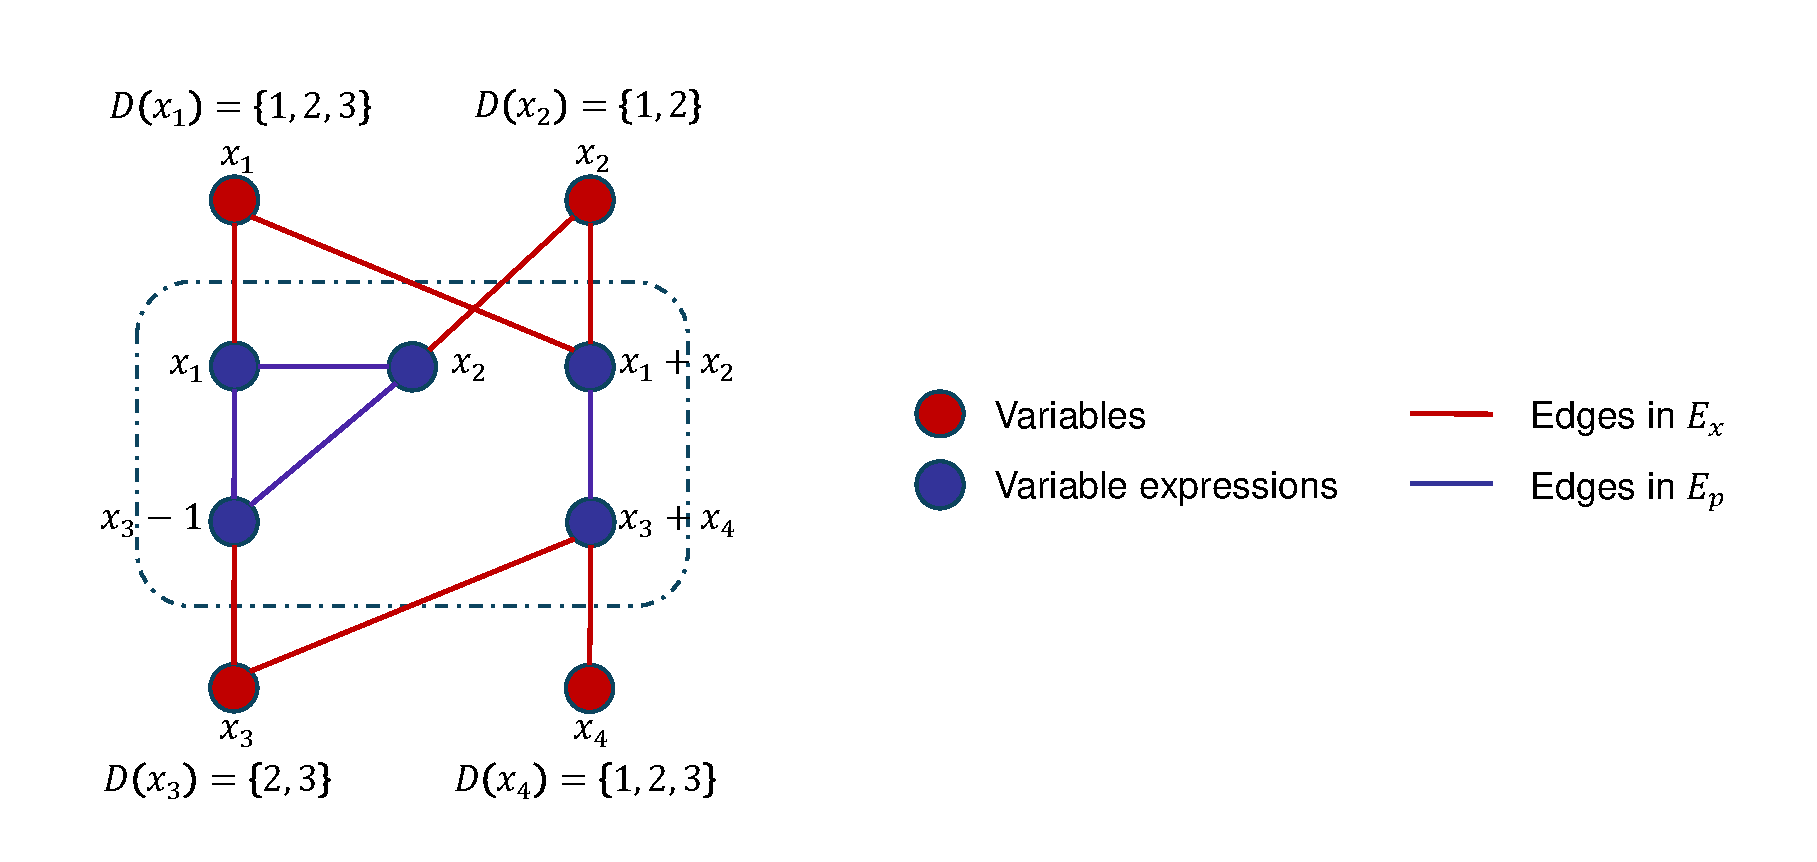
\includegraphics[width=\columnwidth]{Img/acg.pdf}
    \bicaption {例子中约束转化得到约束图。} {The constraints in the example are transformed into a constraint graph.}
    \label{fig:acg}
\end{figure*}

对于得到的ACG,本文需要根据ACG中二元分解得到的二元约束,对变量的值域进行化简。
由于二元约束涉及的变量表达式可能包含多个变量或其他常数,直接套用二元约束的弧一致性算法的效率可能不太理想。
因此,本文根据变量的值域设计了两个化简规则。其核心思想是,对于一个域大小为1的变量$x$(例如,$\{i\}$),可以直接将值$i$分配给$x$,并实施基于二元约束的全局弧一致性检测。同时,在图中,将$x$的变量表达式邻居中相应的变量更改为值$i$,并删除变量顶点$x$及其相关边。
需要注意的是,虽然这些规则以减少ACG中的顶点为主,并不保证整组或单个AllDifferent约束的全局弧一致性。

本文先给出一些基础定义。在ACG中,用$N(x)$表示变量$x$的邻居,用$XN(p)$和$PN(p)$分别表示变量表达式$p$的变量邻居和表达式邻居。
在ACG中,用$N(x)$表示变量$x$的邻居,用$XN(p)$和$PN(p)$分别表示变量表达式$p$的变量邻居和表达式邻居。
在一个CSP中,设$Y = x_{i_1}, x_{i_2}, \dots , x_{i_m}$是一串有限的变量,其中$m > 0$。称一个元组$\mathcal{A}(Y) = (d_{i_1}, d_{i_2}, \dots , d_{i_m}) \in D(x_{i_1}) \times D(x_{i_2}) \times \dots \times D(x_{i_m})$为$Y$的\textit{赋值},并且使用$\mathcal{A}(x)$来表示在赋值$\mathcal{A}$下赋给变量$x$的值。通常,如果一个关于$X$的赋值给出了CSP中的每个变量的赋值,那么它被称为{\it 完整赋值};否则,它就是{\it 部分赋值}。
定义赋值操作如下:
\begin{definition}[\textbf{赋值操作}]
    给定一个变量$x$和一个值$i$,如果将值$i$赋给$x$,那么就意味着在每个$p \in N(x)$中将对应的变量改为值$i$,并在ACG中移除顶点$x$及其相关的边。
\end{definition}

显然,对于值域大小为1的变量$x$(例如,$\{i\}$),可以直接将值$i$赋给$x$。而对于线性单变量表达式$p$(也即,$XN(p) = \{x\}$),$p$的值域与$x$的值域一一对应。
在AllDifferent约束中,这种变量表达式很常见。基于此,本文给出如下两条化简规则,这两条规则可以移除变量的值域中不满足一致性的赋值。
\begin{itemize}
\renewcommand{\labelenumi}{}
    \item \textbf{规则1.} 给定一个约束$c$,设$N(c)$为$c$中包含的表达式,$D(c)$为$\forall p \in N(c)$的可能赋值集的并集。对于一个单变量表达式$p \in N(c)$和一个值$i \in D(c)$,如果$|N(c)| = |D(c)|$,并且$p$是$c$中唯一可以取值$i$的表达式,那么将值$i$赋给$x$。
    \item \textbf{规则2.} 给定一个表达式$p$,若$|XN(p)|$变为0,意味着$p$变成一个常数(例如,$i$)。对于它的一个单变量表达式邻居$q \in PN(x)$(例如,$XN(q)=\{x\}$),如果$i$是$q$的可能赋值,那么从$x$的域中移除使得$q=i$的值。如果$p$的所有邻居都是单变量表达式,那么移除顶点$p$及其相关的边。
\end{itemize}

本文对ACG反复应用两个规则,从而实施赋值操作以减少ACG中的顶点和边。直到ACG中不能再移除任何顶点时,得到最终的ACG。同样的,本文以一个简单的例子介绍化简的过程。
\begin{example}
    对于例\ref{exp:acg}中构造的ACG,考虑约束$c_1$,其中$N(c_1)=\{x_1, x_2, x_3-1\}$和$D(c_1)=\{1, 2, 3\}$。可以通过应用规则1将值3赋给$x_1$,赋值操作会将变量表达式$x_1+x_2$修正为$x_2+3$,变成单变量表达式,同时让表达式$x_1$变为一个常数3,此外变量顶点$x_1$和以它为端点的边也会被删除掉。然后,由于表示常数3的结点的所有邻居都是单变量结点,可以应用规则2删除这个常数顶点和相关的边。ACG的化简过程如图~\ref{fig:simp}所示。
\end{example}

\begin{figure*}[]
    \centering
    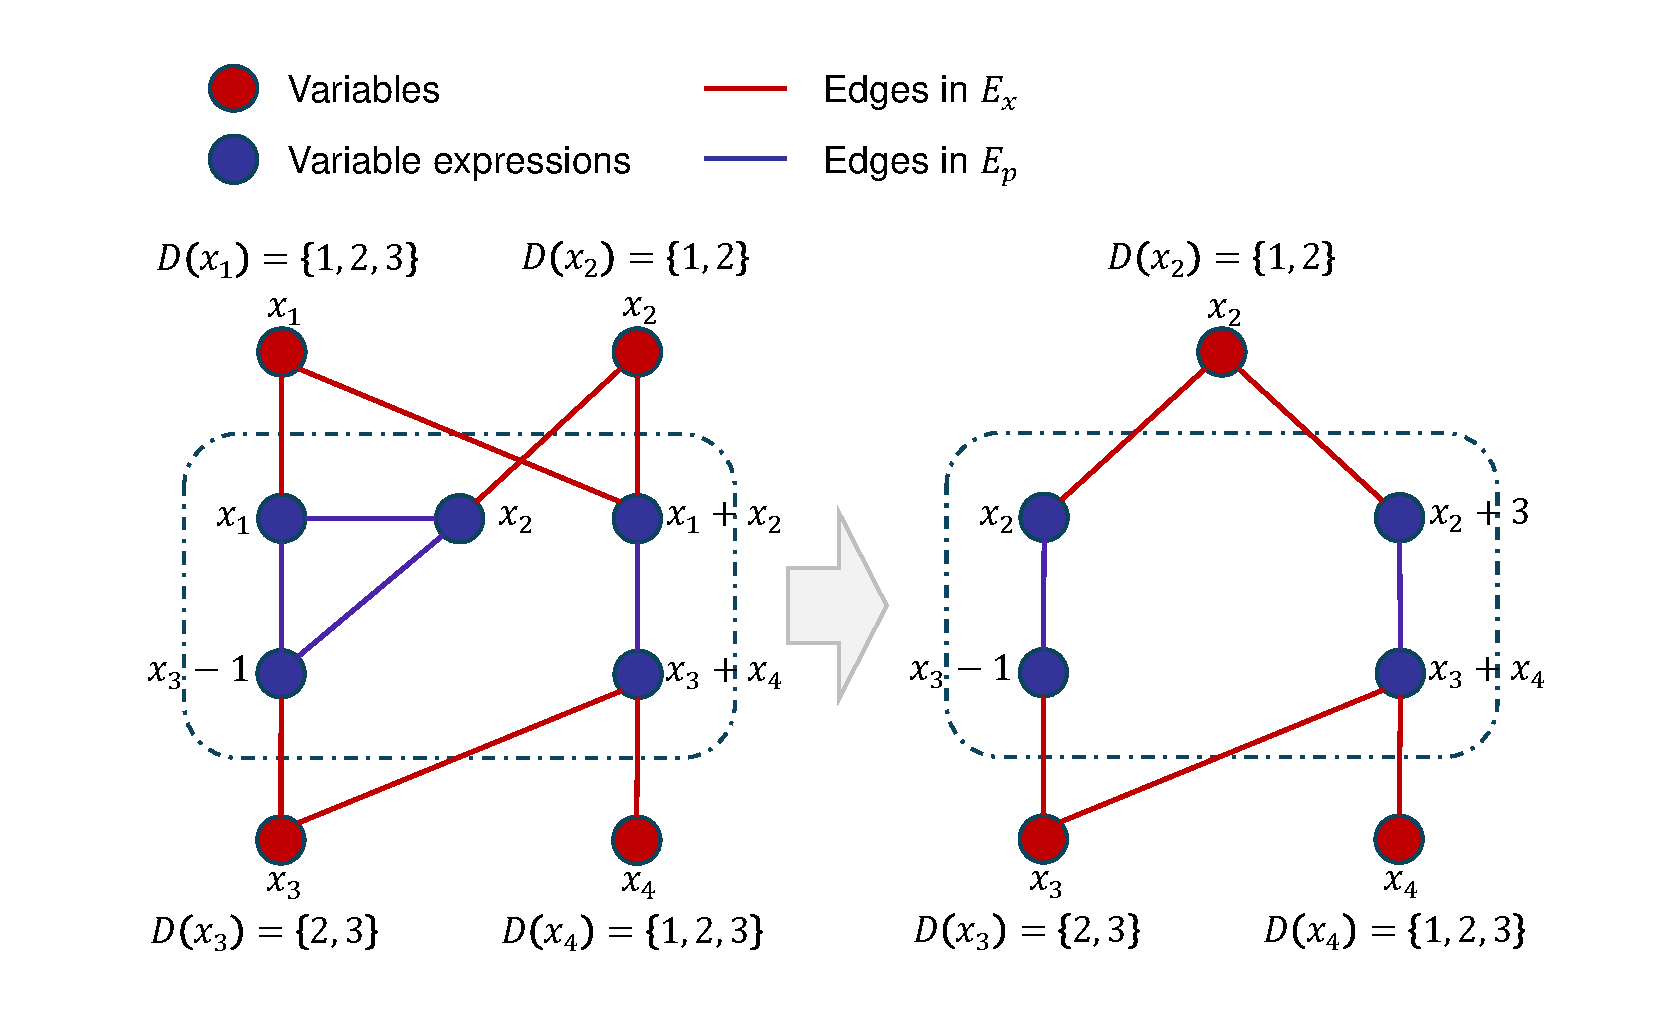
\includegraphics[width=\columnwidth]{Img/simp.pdf}
    \bicaption {例子中约束图的化简。} {Simplification of the constraint graph in the example.}
    \label{fig:simp}
\end{figure*}

对于剩余的变量,他们的值域在后续算法中将不再发生改变。
后面要用到的局部搜索算法需要从一个初始的完整赋值开始,本文选择了随机构造完整赋值的方法。具体来说,对于剩余的变量,从每个变量的域中随机选择一个值作为其赋值。
$Initialization$函数在算法~\ref{alg:init}中给出,第9行是关键步骤。

除此之外,还可以使用针对AllDifferent约束的GAC算法对约束进行过滤,在过滤后再将约束转化为ACG。这种做法对值域的限制较强,保证了每个AllDifferent约束的超弧一致性,但也存在计算复杂度较高等问题。
% 我们采用了最新工作\cite{zhen2023eliminating}中设计的基于二部图匹配的GAC算法,并在实验部分评估了是否使用GAC算法的对算法性能的影响。


\begin{algorithm}[t]
    % \small
    \caption{$Initialization$ function}
    \label{alg:init}
    \textbf{输入}: A CSP $\mathcal{P} = (X, D, C)$ \newline
    % \textbf{Input}: An ACG $\mathcal{G} = (V,E)$ where $V = X\cup NV$ and $E = E_p\cup E_x$, a set of domains $D$\\
    \textbf{输出}: An ACG $\mathcal{G}$ and an complete assignment $\mathcal{A}$
    \begin{algorithmic}[1] %[1] enables line numbers
        \Statex \hrulefill
        \STATE Build an ACG $\mathcal{G} = (V, E)$ for $\mathcal{P}$, where $V = X\cup NV$ and $E = E_p\cup E_x$;
        \STATE $SimpSet \leftarrow \{ x \mid x \in X, |D(x)| = 1 \}$;
        \REPEAT
            \STATE Select a variable $x$ from $SimpSet$ and let $i$ be the unique value in $D(x)$;
            % \STATE $D(x) \leftarrow 0$;
            \FORALL{$v$ in $N(x)$}
                % \STATE replace $x$ contained in $v$ with $i$;
                \STATE Assign $x$ contained in $v$ to $i$;
                % \STATE $d(v) \leftarrow d(v)-1$;
            \ENDFOR
            \STATE Remove $x$ from $X$;
            \STATE Simplify $D$ and $\mathcal{G}$ according to Rule 1 and Rule 2;
            \STATE // Both $V$ and $E$ in $\mathcal{G}$ may potentially be simplified.
            \STATE $SimpSet \leftarrow \{ x \mid x \in X, |D(x)| = 1 \}$;
        \UNTIL{$SimpSet$ is empty}
        \STATE // Initialize $\mathcal{A}$ of $X$ randomly;
        \FORALL{$x$ in $X$}
            \STATE Select a random value $i$ from $D(x)$;
            \STATE $\mathcal{A}(x) \leftarrow i$;
        \ENDFOR
        \STATE \textbf{return} $\mathcal{G}, \mathcal{A}$;
    \end{algorithmic}
\end{algorithm}

\section{分步选择操作策略}
% 先介绍启发式策略CBLS
在局部搜索中,一个移动(又称操作)意味着对赋值进行轻微的修改,它定义了候选解的邻域。一般来说,移动的复杂性应尽可能地保持低,同时确保它能够充分探索当前解的邻域。
在启发式的局部搜索框架CBLS(Constraint-Based Local Search,基于约束的局部搜索)中,会先满足部分AllDifferent约束,之后通过交换约束中两个变量的赋值的操作实现对当前状态的修改,这里提到的交换操作称为$swap$,就是一种移动。

相对的,本文采用的是一个简单但有效的操作符$mov$,它通过将一个变量顶点的值修改为其值域中的其他值的方式来修改当前的完全赋值,上面提到的交换操作相当于对交换的两个变量分别作了一次修改赋值的操作$mov$。这样做的动机是$mov$相较于$swap$对约束修改的粒度更细,使得其邻域范围更广,能够实现更快的收敛速度,实际上,实验也表明了$swap$移动在求解包含复杂AllDifferent约束的CSP时存在困难。下面是$mov$的形式化定义。

\begin{definition}
给定一个变量顶点$x$和一个值$i$,将$x$的值从$\mathcal{A}(x)$改变为$i$的操作符定义为$mov(x, i)$。
\end{definition}

对于每个$(p,q) \in E_p$,如果$\mathcal{A}(p) = \mathcal{A}(q)$,称$(p,q)$为{\it 冲突边}。对于一个ACG $\mathcal{G}$,一个完整赋值$\mathcal{A}$的代价,表示为$cost(\mathcal{G},\mathcal{A})$,是在$\mathcal{A}$下的冲突边的总数。本文采用ACG中冲突边的改进数量,作为$mov$的度量,因此一个$mov$的打分函数可以表示为%
\begin{align}
    score(mov) = cost(\mathcal{G}, \mathcal{A}) - cost(\mathcal{G}, \mathcal{A}'),
\end{align}%

其中$\mathcal{A}'$是通过在$\mathcal{A}$上应用$mov$获得的。
本文使用$cost(x, i)$来表示将值$i$赋给$x$的代价,即当$\mathcal{A}(x) = i$时,以$\forall y \in N(x)$为终点的冲突边的总数。
由于$mov(x, i)$只影响那些以$x$的邻居为终点的边,所以$mov(x, i)$的冲突分数可以由$x$的改变代价来表示,定义如下:

\begin{definition}
给定一个ACG $\mathcal{G}$,操作符$mov(x, i)$的冲突分数定义为
\begin{align}
    score(mov) = cost(x, \mathcal{A}(x)) - cost(x, i).
\end{align}%
\end{definition}

通常人们倾向于通过反复选择最合适的$mov$,不断降低$\mathcal{G}$在$\mathcal{A}$下的冲突边数,也即$cost(\mathcal{G}, \mathcal{A})$,直到找到一个解。一个最常见的贪心选择准则是选择使得$score(mov)$最大的$mov$,这个方法叫做\textit{爬山法},它是很多启发式算法的基础。

在选择操作符时,需要确保它不会陷入循环,并且能在考虑约束条件的满足情况下逃离局部最优。
给定一个变量$x$,本文用$mc(x)=min(\{ cost(x, i) \mid i \in D(x)/A(x) \})$表示$x$在除当前赋值外的所有可能赋值下的最小$cost$。
基于此,本文定义一个变量集$X'=\{ x \mid cost(x, \mathcal{A}(x)) \geq mc(x), x \in X \}$,称为\textit{候选变量集},它拥有一个重要的性质:对于$X'$中的每个变量,都有至少一个$mov$保证冲突边的数量不会增加。
考虑到$mov$包含两部分:变量和值,本文提出以下\textit{两步选择策略}:
\begin{itemize}
    \item \textbf{步骤1.} 从$X'$中选择在$\mathcal{A}(x)$下具有最高$cost$的变量$x$;
    \item \textbf{步骤2.} 从$D(x)$中选择使所选$x$的$cost$最小的值$i$。
\end{itemize}

在依次选择变量$x$和值$i$后,已经确定了要执行的$mov(x, i)$。虽然两步选择可能会错过一些更贪婪的$mov$(在第一步未被选择的变量可能有更好的赋值),但它可以大大降低选择$mov$的时间复杂度。
设$|D|$表示每个变量的平均值域的大小,那么直接的$mov$选择方法需要$|X| \cdot |D|$的复杂度,而两步$mov$选择只需要$|X| + |D|$的复杂度,从而降低了最坏情况下的时间成本。此外,候选变量集$X'$确保了所选变量的下限质量。

然而,局部搜索算法经常会陷入局部最优,这意味着$X'$是空的。在这种情况下,本文定义了一个新的候选变量集$X''$,它表示当前存在冲突的变量集,称为\textit{冲突变量集}。这个变量集的动机来自于改变没有冲突的变量的赋值不会减少冲突的总数。$X''$不能保证变量的质量,所以在这种情况下,本文直接选择$score$最大的$mov$,$mov$中的$x$只能从$X''$中选择。为了和两步选择策略有所区分,本文称这种选择方式为\textit{直接选择策略}。

\section{禁忌策略}
局部搜索算法使用{\it 禁忌策略} \cite{glover1998tabu}来避免陷入循环。
鉴于需要通过两步来选择操作,本文提出了一个禁忌策略组合,包括以下策略。

\begin{itemize}
    \item \textbf{策略1.} 在一个变量表达式改变其值后,它将被禁忌,直到出现一个以它为端点的新的冲突边。此外,如果一个变量的所有邻居都被禁忌,那么该变量也将被禁忌;
    \item \textbf{策略2.} 在一个变量$x$被赋予值$i$后,接下来的$tt$次迭代中,操作$mov(x,i)$将被禁忌,其中$tt$是一个被称为{\it 禁忌期限}的参数;
    \item \textbf{策略3.} 如果选择的$mov$被禁忌的同时其变量也被禁忌,那么算法在接下来的$\beta$步中切换到直接选择策略。
\end{itemize}

在算法的求解流程中,策略1在变量选择阶段实施。策略3确保算法在两步选择策略的性能下降时,能够快速切换到直接选择策略。在直接选择中,只使用策略2。接下来,本文将具体介绍这三个策略的动机和细节。

% 策略一,改良版格局检测,介绍格局,介绍原因。
策略1可以看作是一种\textit{格局检测策略}\cite{cai2011local}的变体,它最初是为了解决最小顶点覆盖问题中局部搜索算法的循环问题而被设计出来的,并在此后应用在许多图论问题上。格局检测策略的核心目标是在向当前候选解添加点时考虑该点的邻域。
在本文中,本文用$S_x$表示关于变量的禁忌表,它初始为空。在选择一个操作$mov(x,i)$执行时,会同步地将变量$x$放入$S_x$中,在禁忌表中的变量在第一阶段选择变量时不会被选中,除非$S_x = X'$,也即所有变量都在禁忌表中。
基于此,本文定义一个变量的\textit{格局}如下:

\begin{definition}[格局]
对于ACG中的一个变量顶点$x$,其格局定义为其所有邻居的状态向量 $F_v$。其中,一个变量表达式顶点的状态表示为 $f_p \in \{0, 1\}$,具体地:
\[
f_p = 
\begin{cases} 
1, & \text{若出现新的以$p$为端点的冲突边;}\\
0, & \text{其他情况.}
\end{cases}
\]
\end{definition}
如果把变量表达式的格局定义为其与其变量表达式邻居构成的边,那么变量的格局可以视为变量表达式格局构成的格局,形成嵌套关系。
一个变量的格局发生改变,当且仅当它所关联的变量表达式的格局发生改变。在$S_x$中的变量的格局改变时,会从$S_x$中移除该变量。
这种策略是合理且直观的,因为它避免了重复选取同一个变量导致的循环情况。

% 策略二,传统的tabu策略,介绍tabu策略的思想。
然而,在实际求解过程中发现,仅采用策略一时仍然会发生循环。考虑如下场景:两个相关联的变量对应的$mov$会互相改变对方的格局,在不限制$mov$的情况下,一个变量在被禁忌后会被另一个变量对应的$mov$激活,导致两个$mov$被无限循环地选择。基于此,本文构造了关于变量值域的禁忌表$S_m$,采用传统的tabu策略维护$S_m$。该策略基于以下思路:通过禁止对最近的变化进行反转,避免局部搜索马上返回刚刚访问过的状态进而导致循环。在算法求解时,本文在选择一个$mov$时,会优先选择没有被禁忌的变量,并优先从变量的值域中选择没有被禁忌的赋值。

% 策略三,什么情况下会发生这种情况,以及这样的效果。
在应用策略1和策略2时,需要注意到,在执行一个操作后,该操作在被禁忌的同时可能无法从禁忌表中激活任何变量。
因此,禁忌搜索可能会出现如下情况:在两步选择策略中,会出现所有变量都被禁忌的情况。这种情况往往发生在局部搜索趋于稳定的后期。

考虑一种极端情况,在两步选择策略中,若所有$X'$中的变量都被禁忌,在步骤一中将不得不从禁忌表里选择一个变量$x$,而恰好变量$x$的所有赋值也都被禁忌,导致在步骤二中还需要从禁忌表中选择一个被禁忌的赋值$i$。
在这种情况下,会得到一个被双重禁忌的操作$mov(x,i)$。一个更合理的策略是,直接切换到直接选择策略,通过更贪心的选择策略寻找当前状态的邻域下最合适的操作。因此,本文设计了策略3,它实际上是一种快速转换机制,作为前面提到的根据冲突变量集$X''$切换的补充。

\section{打破平局策略}
另一方面,由于AllDifferent约束的性质,在直接选择$mov$时,经常有许多最大$score$的$mov$不唯一的情况。常用的打破平局策略有随机选择策略、子打分函数策略等。其中,随机选择策略会在所有具有相同优化目标值的解决方案中随机选择一个;而子打分函数策略除了主要的打分函数外,还会设计子打分函数。当且仅当通过主打分函数得到的最优操作有多个时,我们会使用子打分函数进行评分和排序,以此来打破平局。

本文提出了一个新的$nscore$作为$score$的补充,它利用了变量的邻域信息。如果两个变量的邻居之间存在冲突边,就说这两个变量处于冲突中。本文使用$n(x, i)$来表示当值$i$被赋予$x$时,与$x$冲突的变量的数量。

\begin{definition}
给定一个ACG $\mathcal{G}$,一个$mov(x,i)$的$nscore$定义为 
\begin{align}
    % nscore(mov) = {\sum_{u \in CN(x, \mathcal{A}(u))} {cost(u, \mathcal{A}(u))}} - {\sum_{u \in CN(x, i)} {cost(u, \mathcal{A}(u))}}.
    nscore(mov) = n(x, \mathcal{A}(x))  - n(x, i).
\end{align}%
\end{definition}

与$score$相比,$nscore$关注的是变量之间的冲突,由于在ACG中的侧重点不同,一个$mov$在两个打分机制下不会出现高度相似的现象,从而保证打破平局的有效性。下面通过一个例子介绍该打分函数如何起作用。

\begin{example}\label{exp:nscore}
考虑\figurename~\ref{fig:simp}右图所示的ACG示例,并假设它当前在赋值$\mathcal{A} = (1, 2, 2)$下。那么$score(mov(x_2, 2)) = score(mov(x_3, 3)) = 2$,而$nscore(mov(x_2, 2)) = 2$和$nscore(mov(x_3, 3)) = 1$。因此,选择执行$mov(x_2, 2)$。
\end{example}

最终的评价准则如下:首先通过打分函数$score$寻找评分最高的$mov$,在$mov$不唯一时,使用更细粒度的子打分函数$nscore$对$mov$进行评价,优先选择$nscore$最大的$mov$打破平局,若$mov$仍然不唯一,通过随机选择的方式打破进一步的平局。在本节的最后,本文给出最终的$SelectMove$函数,如算法~\ref{alg:selectMove}所示。它最初采用两步选择策略,当$X'$为空时,接下来的$\beta$步将使用直接选择策略,其中$\beta$是用于控制步长的常数。

\begin{algorithm}[t]
    % \small
    \caption{$SelectMove$ function}
    \label{alg:selectMove}
    \textbf{输入}: A complete assignment $\mathcal{A}$, a control variable $mode$ and candidate variable sets $X', X''$\newline
    \textbf{输出}: A variable $x$ and a value $i$
    \begin{algorithmic}[1] %[1] enables line numbers
        \Statex \hrulefill
        \IF {$mode = 0$}
            % \STATE Calculate candidate variable set $X'$;
            \STATE Select a variable $x$ from $X'$ based on $cost(x, \mathcal{A}(x))$ and Strategy 1; 
            \STATE Select a value $i$ from $D(x)$ based on $cost(x, i)$ and Strategy 2;
            \IF {$x$ is Tabu and $mov(x,i)$ is Tabu}
                \STATE $mode \leftarrow \beta$; // Strategy 3
                \STATE Initialize $X''$ according to $\mathcal{A}$;
                % \STATE Initialize $mc(x)$ for $\forall x \in X$;
            \ENDIF
        \ELSE
            \STATE Select $x$ from $X''$ and $i$ based on $score(mov)$ and $nscore(mov)$;
            \STATE $mode \leftarrow mode - 1$;
        \ENDIF \\
        \RETURN $x, i$
    \end{algorithmic}
\end{algorithm}

\section{局部搜索算法框架}

\begin{figure*}[]
    \centering
    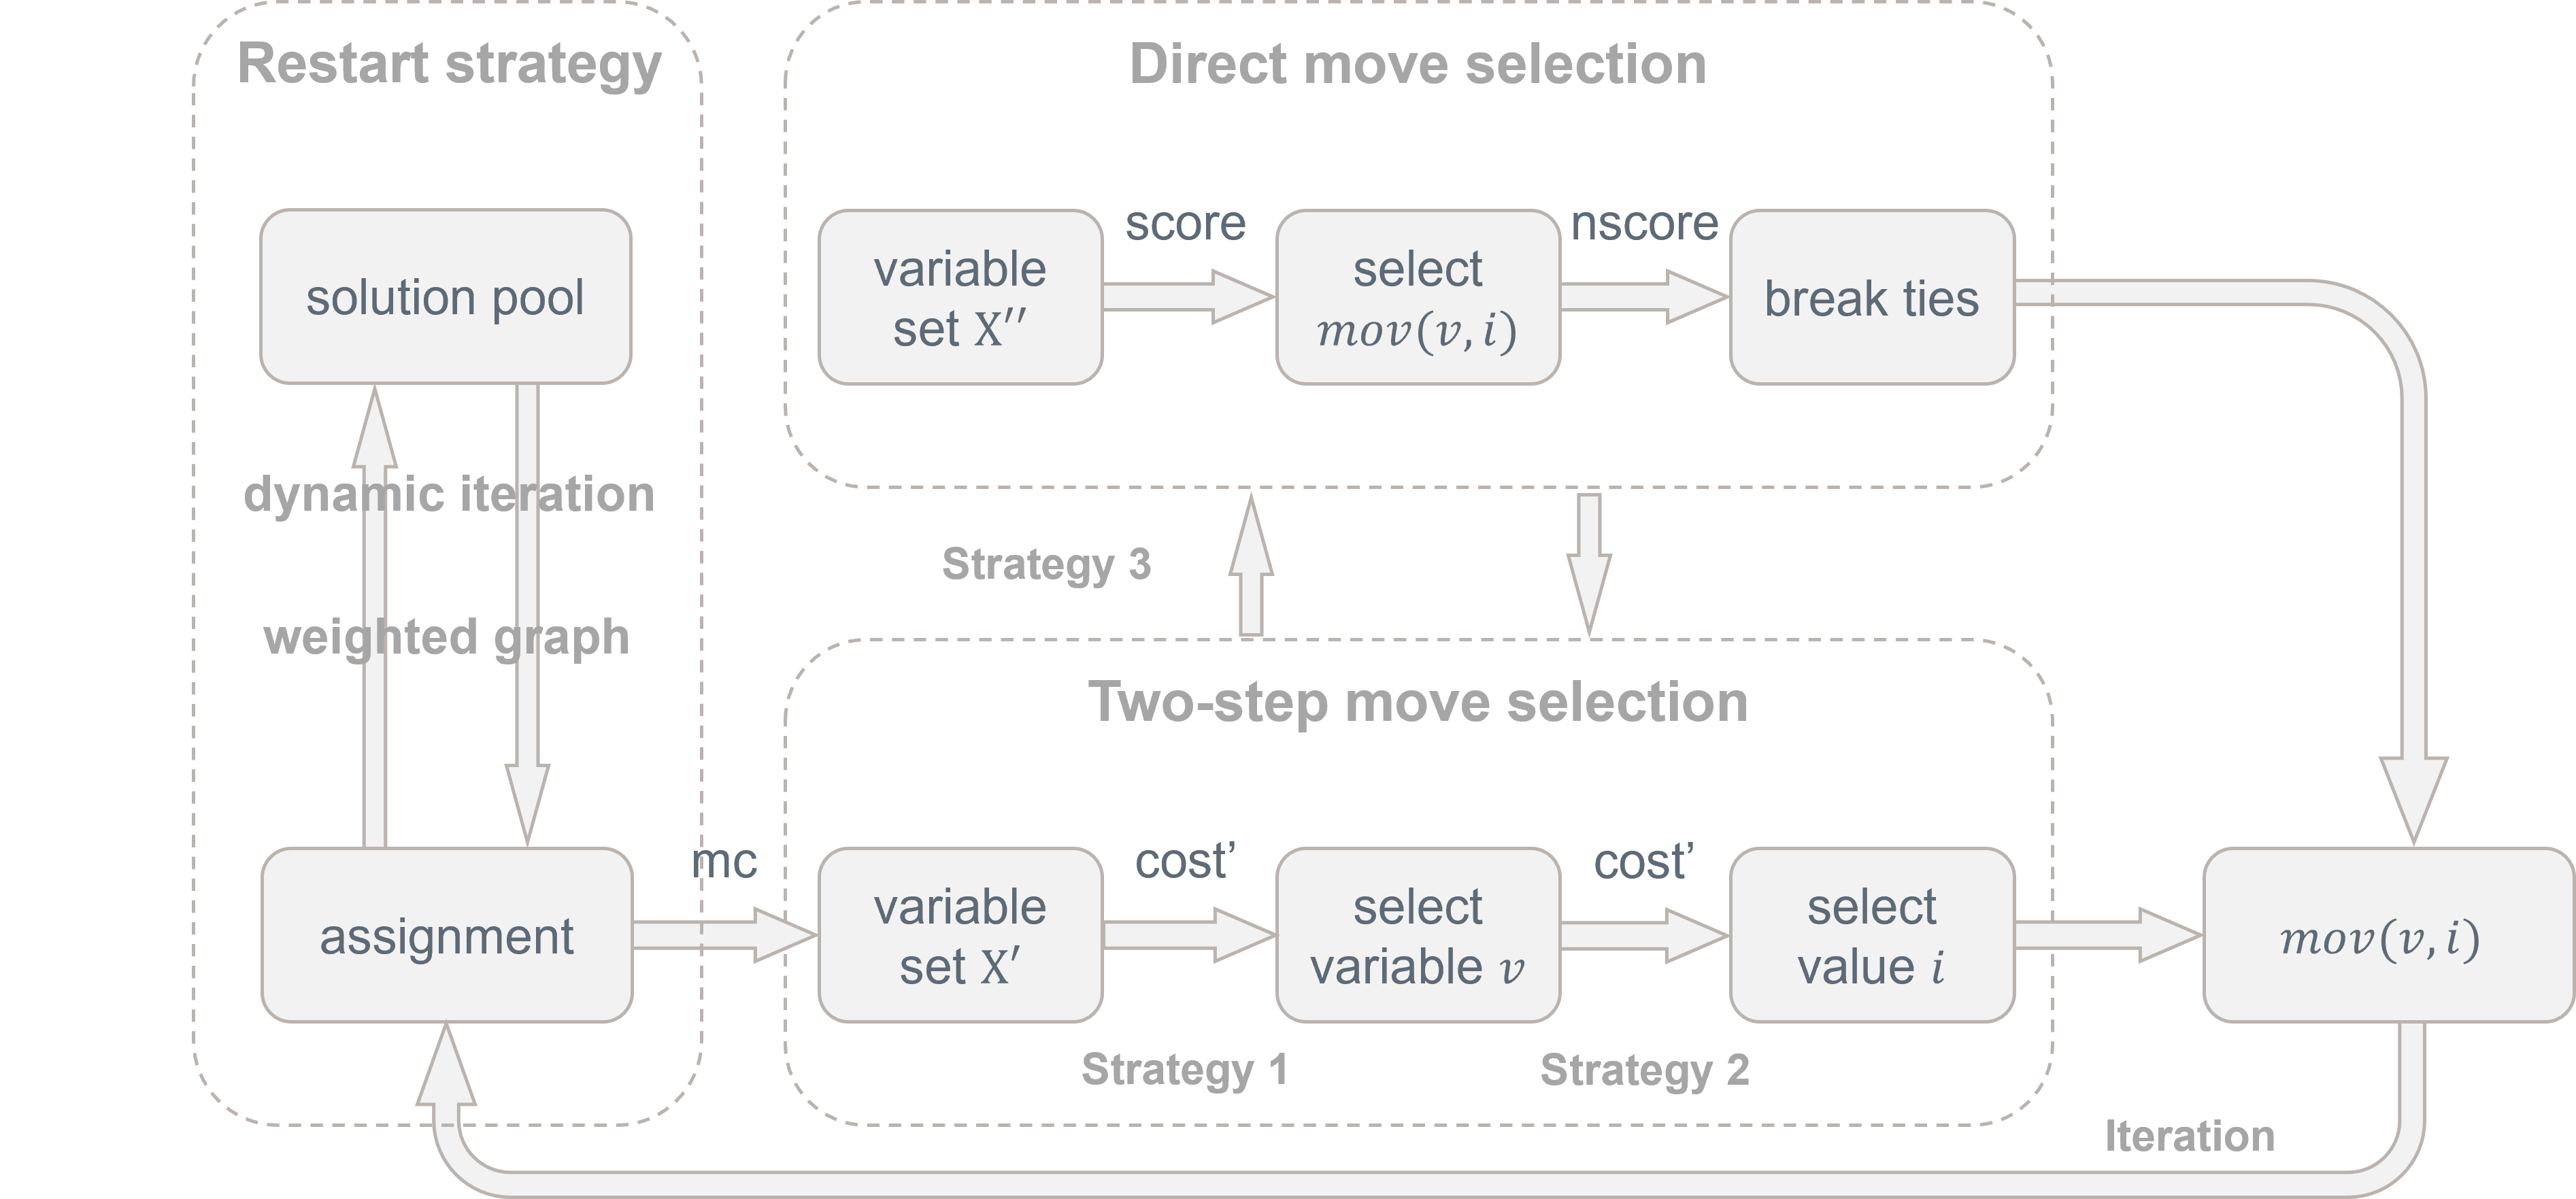
\includegraphics[width=\columnwidth]{Img/total.png}
    \bicaption {Local Search的求解流程。} {The solving process of Local Search.}
    \label{fig:acls}
\end{figure*}

在构造了状态、打分函数、邻域以及评价准则后,可以得到构造一个局部搜索算法所需的基本框架。基于前几节提到的定义和策略,本文设计了一个用于解决包含AllDifferent约束问题的CSP的局部搜索算法,称为AllDiff-LS。算法的主体部分如\figurename~\ref{fig:acls}所示,算法采用了迭代局部搜索的框架,主要由三个部分组成,即两步选择策略、直接选择策略和重启策略,本章中已经介绍了前两个部分,重启策略部分将在下一章进行介绍。

\begin{algorithm}[h]
    % \small
    \caption{AllDiff-LS algorithm}
    \label{alg:AllDiff-LS}
    \textbf{输入}: A CSP $\mathcal{P} = (X, D, C)$ and time limit $T$\newline
    \textbf{输出}: A complete assignment $\mathcal{A}_b$
    
    \begin{algorithmic}[1] %[1] enables line numbers
        \Statex \hrulefill
        \STATE Initialize $\mathcal{G}, \mathcal{A}$; 
        \STATE $\mathcal{AC} \leftarrow []$;
        \STATE $maxIter \leftarrow \alpha$;
        % \STATE Initialize a complete assignment $\mathcal{A}$ randomly;
        \REPEAT
            % \STATE Initialize a conflict vertex set $V_c$ based on $\mathcal{A}$;
            \STATE Initialize $mc(x)$ for $\forall x \in X$;
            \STATE Initialize $X'$ according to $mc(x)$ and $\mathcal{A}$;
            \STATE $mode \leftarrow 0$;
            \STATE $\mathcal{A}_b \leftarrow \mathcal{A}$;
            \IF {$X' = []$}
                \STATE Initialize $X''$ according to $\mathcal{A}$, $mode \leftarrow \beta$; 
            \ENDIF
            \REPEAT
                \STATE $x,i \leftarrow SelectMove(\mathcal{A}, mode, X', X'')$;
                \STATE $\mathcal{A}(x) \leftarrow i$;
                \STATE Update $mc(x)$, update $X'$ or $X''$;
                \IF {$mode > 0$ \textbf{and} $X' = \emptyset$}
                    \STATE Initialize $X''$ according to $\mathcal{A}$;
                    \STATE $mode \leftarrow \beta$; 
                \ENDIF
                % \STATE update tabu list and conflict vertex set $V_c$;
                \IF {$cost(\mathcal{G}, \mathcal{A}) \leq cost(\mathcal{G}, \mathcal{A}_b)$}
                    \STATE $\mathcal{A}_b \leftarrow \mathcal{A}$;
                \ENDIF
                \STATE $iter \leftarrow iter + 1$; 
            \UNTIL{$iter \geq maxIter$}
            \IF {$cost(\mathcal{G}, \mathcal{A}_b) = 0$}
                \RETURN $\mathcal{A}_b$
            \ENDIF
            \STATE $\mathcal{A} \leftarrow SelectSolution(\mathcal{G}, \mathcal{A}_b, \mathcal{AC})$;
            \STATE $maxIter \leftarrow \mathcal{A}.step$;
        \UNTIL{$T$ is reached}
        \STATE \textbf{return} $\emptyset$
    \end{algorithmic}
\end{algorithm}

本文在算法~\ref{alg:AllDiff-LS}中给出了方法的伪代码描述。
AllDiff-LS算法的输入是一个仅包含AllDifferent约束的CSP $\mathcal{P} = (X, D, C)$ 以及一个时间限制$T$,输出则是一个关于输入的CSP的完整赋值$\mathcal{A}_b$。
首先,本文使用前述的初始化算法~\ref{alg:init}随机生成了一个初始的完整赋值$\mathcal{A}$。接下来,算法以迭代的方式运行,包含一个外循环和一个内循环。注意,内循环由最大迭代次数$maxIter$(第24行)控制,而外循环由截止时间$T$(第29行)控制。

在内循环(第13-23行)中,算法搜索具有最小代价的完整赋值。算法首先通过$SelectMove$函数获取一个操作$mov$,然后实施$mov$,同时更新两个禁忌列表$S_x$和$S_m$,以及有冲突的顶点。每个内循环结束后,下一轮的初始完整赋值和最大迭代次数将通过$SelectSolution$(第27-28行,下一章介绍)获得。如果在给定的时间限制$T$内找到了一个没有冲突的完整赋值,那么返回该赋值(第25行);否则,返回一个空集(第30行)。

\section{本章小结}

本章节将CSP转化为了图结构,并设计了一个用于求解此类问题的局部搜索算法,具体如下。
在第一节中,本文给出了要研究的问题,以AllDifferent约束为主的CSP的形式化定义。
在第二节中,本文将CSP中包含的AllDifferent约束转化为约束图,并设计了两个化简规则对约束进行化简。
在第三节中,本文介绍了分两步选择操作的策略,作为直接选择操作策略的补充。
在第四节中,本文设计了局部搜索的禁忌搜索框架。
在第五节中,本文设计了包含打破平局策略的操作评价准则。
在第六节中,本文将前面提到的策略整合在了一起,实现了局部搜索算法:AllDiff-LS,并介绍了算法的流程细节。
